\documentclass[handout]{beamer}
\definecolor{lmu@green}{rgb}{0,0.58,0.25} % use structure theme to change
\definecolor{lmu@darkgreen}{rgb}{0,0.4,0.12} % use structure theme to change
% Uncomment the following for handouts.
%\documentclass[handout]{beamer}
\usepackage[utf8x]{inputenc}
\usepackage{amsmath,amsfonts,amssymb}
\setbeamertemplate{navigation symbols}{}

% Python listing setup

\usepackage{color}
\usepackage[procnames]{listings}
\usepackage{textcomp}
\usepackage{setspace}
\usepackage[]{xcolor}
\definecolor{gray}{gray}{0.5}
\definecolor{green}{rgb}{0,0.5,0}
\definecolor{lightgreen}{rgb}{0,0.7,0}
\definecolor{purple}{rgb}{0.5,0,0.5}
\definecolor{darkred}{rgb}{0.7,0,0}

\lstnewenvironment{python}[1][]{
\lstset{
% Escape with funnyeyes.
escapeinside={(*@}{@*)},
language=python,
basicstyle=\ttfamily\small,
stringstyle=\color{green},
showstringspaces=false,
alsoletter={1234567890},
otherkeywords={\ , \}, \{},
keywordstyle=\color{blue},
emph={access,and,as,break,class,continue,def,del,elif,else,%
except,exec,finally,for,from,global,if,import,in, is,%
lambda,not,or,pass,print,raise,return,try,while,assert},
emphstyle=\color{orange}\bfseries,
emph={[2]self},
emphstyle=[2]\color{gray},
emph={[4]ArithmeticError,AssertionError,AttributeError,BaseException,%
DeprecationWarning,EOFError,Ellipsis,EnvironmentError,Exception,%
False,FloatingPointError,FutureWarning,GeneratorExit,IOError,%
ImportError,ImportWarning,IndentationError,IndexError,KeyError,%
KeyboardInterrupt,LookupError,MemoryError,NameError,None,%
NotImplemented,NotImplementedError,OSError,OverflowError,%
PendingDeprecationWarning,ReferenceError,RuntimeError,RuntimeWarning,%
StandardError,StopIteration,SyntaxError,SyntaxWarning,SystemError,%
SystemExit,TabError,True,TypeError,UnboundLocalError,UnicodeDecodeError,%
UnicodeEncodeError,UnicodeError,UnicodeTranslateError,UnicodeWarning,%
UserWarning,ValueError,Warning,ZeroDivisionError,abs,all,any,apply,%
basestring,bool,buffer,callable,chr,classmethod,cmp,coerce,compile,%
complex,copyright,credits,delattr,dict,dir,divmod,enumerate,eval,%
execfile,exit,file,filter,float,frozenset,getattr,globals,hasattr,%
hash,help,hex,id,input,int,intern,isinstance,issubclass,iter,len,%
license,list,locals,long,map,max,min,object,oct,open,ord,pow,property,%
quit,range,raw_input,reduce,reload,repr,reversed,round,set,setattr,%
slice,sorted,staticmethod,str,sum,super,tuple,type,unichr,unicode,%
vars,xrange,zip},
emphstyle=[4]\color{purple}\bfseries,
upquote=true,
morecomment=[s][\color{lightgreen}]{"""}{"""},
commentstyle=\color{red}\slshape,
literate={>>>}{\bfseries{\textcolor{darkred}{>{>}>}}}3%
         {...}{{\textcolor{gray}{...}}}3,
procnamekeys={def,class},
procnamestyle=\color{blue}\textbf,
framexleftmargin=1mm, framextopmargin=1mm,
rulesepcolor=\color{blue},#1
}}{}



\usetheme{LMU}
\usecolortheme{lmu}
\useinnertheme{lmu}
\useoutertheme{lmu}

% -----------------------------------------------------------------------------
%
%\newtheorem{definition}{Definition}
\newcommand{\foot}[1]{_{\mbox{\footnotesize #1}}}
\newcommand{\head}[1]{^{\mbox{\footnotesize #1}}}
%
%
\newcommand{\ones}{\mathbb{I}}
\newcommand{\nat}{\mathbb{N}}
\newcommand{\real}{\mathbb{R}}
\newcommand{\ganz}{\mathbb{Z}}
%
%
\newcommand{\RRE}{\mbox{RRE}}
\newcommand{\nnz}[1]{\mbox{nnz}(#1)}
\newlength{\Hoehe}
\renewcommand{\vec}[1]{#1}
\newlength{\GLaenge}
\setlength{\GLaenge}{3.5cm}
%
%
\definecolor{MyGrey}{gray}{0.45}
\def\bstheta{\boldsymbol{\theta}}
\def\bsalpha{\boldsymbol{\alpha}}
\def\bsk{\boldsymbol{k}}
\def\bsx{\boldsymbol{x}}
\def\bsh{\boldsymbol{h}}
%
% Centred minipage environment
%
\newenvironment{cmpage}[1]{
\begin{center}
\begin{minipage}{#1\textwidth}}%
{\end{minipage}\end{center}}
%
%
\newcommand{\POS}{\color{blue}\item [\boldmath{$+$}]}
\newcommand{\NEG}{\color{red}\item [{\boldmath$-$}]}
\newcommand{\NTR}{\color{black}\item [$\circ$]}
\newcommand{\f}[1]{\mathfrak{#1}}
\newcommand{\old}{^{\mbox{\small \color{blue} old}}}
\newcommand{\new}{^{\mbox{\small \color{red} new}}}
\newcommand{\diag}[1]{\mbox{diag}\left(#1\right)}
%
%
\newcommand{\myBlank}{\textvisiblespace}
\newcommand{\noSpace}{\makebox[0pt]{\quad}}
%
% Old style colour commands
%
\newcommand{\CB}{\color{blue}}
\newcommand{\CR}{\color{red}}
\newcommand{\CG}{\color{green}}
\newcommand{\CC}{\color{cyan}}
%
\definecolor{myWhite}{rgb}{1.00,1.00,1.00}  % real white
\definecolor{myGrey}{rgb}{0.78,0.83,0.94}   % 'light grey blue'
\definecolor{myYellow}{rgb}{1.00,1.00,0.00} % yellow
\definecolor{myOrange}{rgb}{1.00,0.65,0.00} % orange
\definecolor{myCyan}{rgb}{0.00,1.00,1.00}   % cyan
%
% Some abbrevs for setting brief code parts
%
\newcommand{\ttA}{\mbox{\texttt{A}}}
\newcommand{\ttB}{\mbox{\texttt{B}}}
\newcommand{\ttC}{\mbox{\texttt{C}}}
\newcommand{\ttD}{\mbox{\texttt{D}}}
\newcommand{\code}[1]{\mbox{\texttt{#1}}}
\newcommand{\ccode}[1]{\cemphd{\texttt{#1}}}
%
% Commands for slides taken from 'Insides'
%
\newcommand{\rst}{\textcolor{emphcolora}{\ast}}
\newcommand{\bst}{\textcolor{emphcolorb}{\ast}}
%
%
%
\definecolor{textcolor} {rgb}{0,0,0}
\definecolor{decocolor} {rgb}{0,0,0}
\definecolor{emphcolora}{rgb}{1,0,0}              % pure red
\definecolor{emphcolorb}{rgb}{0,0,1}              % pure blue
\definecolor{emphcolorc}{cmyk}{0,1,0,0}           % pure magenta
%\definecolor{emphcolord}{cmyk}{0.64,0,0.95,0.20} % sort of green
\definecolor{emphcolord}{rgb}{0,0.4,0.12}         % same as lmu@darkgreen
\definecolor{emphcolore}{cmyk}{1,0,0,0}           % pure cyan
\definecolor{linkcolor} {rgb}{0,0,0}
%
% Commands emphasising text using color
%
\newcommand{\cempha}[1]{{\color{emphcolora}#1}}
\newcommand{\cemphb}[1]{{\color{emphcolorb}#1}}
\newcommand{\cemphc}[1]{{\color{emphcolorc}#1}}
\newcommand{\cemphd}[1]{{\color{emphcolord}#1}}
\newcommand{\cemphe}[1]{{\color{emphcolore}#1}}
\newcommand{\cemphf}[1]{{\color{decocolor}#1}}
% -----------------------------------------------------------------------------
% myColorBox
% -----------------------------------------------------------------------------
\setbeamercolor{myBoxColor}{fg=black,bg=white}
\setbeamercolor{myBoxColorHead}{fg=red,bg=white}
% \newenvironment{myColorBox}[2]{%
% \begin{beamerboxesrounded}[shadow=true,lower=myBoxColor,upper=myBoxColorHead,
% width=#1\textwidth]{#2}}%
% {\end{beamerboxesrounded}}
\newenvironment{myColorBox}[2]{%
\begin{cmpage}{#1}%
\begin{beamerboxesrounded}[shadow=true,lower=myBoxColor,upper=myBoxColorHead]%
{#2}}%
{\end{beamerboxesrounded}\end{cmpage}}
%
% -----------------------------------------------------------------------------
% Math Operators, alternate greek symbols and the like
% -----------------------------------------------------------------------------
\DeclareMathOperator{\grad}{grad}
\DeclareMathOperator{\mydiv}{div}
\DeclareMathOperator{\Grad}{grad}
\DeclareMathOperator{\Div}{div}
%\newcommand{\grad}{\mbox{grad}}
%\newcommand{\mydiv}{\mbox{div}}
\renewcommand{\rho}{\varrho}
%
% -----------------------------------------------------------------------------
% Some color defintions to be compatible with XFIG
% -----------------------------------------------------------------------------
%
\definecolor{XFIGgold}{rgb}{1.00,0.84,0.00}
\definecolor{XFIGltblue}{rgb}{0.53,0.81,1.00}
\definecolor{XFIGred}{rgb}{1.00,0.00,0.00}
% -----------------------------------------------------------------------------

\usepackage{lmodern}

% Meta information.
\subtitle{ObsPy Workshop at IPGP}
\author{Lion Krischer}
\date{Paris, Feb 21-22 2013}
\institute[LMU]{Ludwig-Maximilians-University in Munich\\ Department of Earth and Environmental Sciences\\ Geophysics}
\title{First Steps in ObsPy}


\begin{document}

\frame[plain]{\titlepage}

\begin{frame}[plain, fragile]{}
    \begin{center}
        \textcolor{lmu@darkgreen}{\LARGE{Introduction to ObsPy}}
    \end{center}
\end{frame}


\begin{frame}[plain]{What is ObsPy and what can it do}
    A Python Toolbox for seismology/seismological observatories.

    \vspace{2em}

    The goal of the ObsPy project is to \textbf{facilitate rapid application development for seismology}.

    \vspace{3em}

    \large
    \begin{center}
        \textbf{http://www.obspy.org}
    \end{center}
\end{frame}


\begin{frame}[plain, fragile]{What is ObsPy and what can it do}
    \begin{itemize}
        \item In development since 2008
        \item 6 core developers
        \item Many more people contribute
        \item Thoroughly unit tested
        \item Written in Python (performance critical parts are written in C)
        \item Uses well established libraries (libmseed, GSE\_UTI, \dots)
        \item Open source and cross platform
        \item Starts to get widely used in the community
    \end{itemize}
\end{frame}


\begin{frame}[plain, fragile]{What is ObsPy and what can it do}
    \begin{itemize}
        \item \textbf{Read and write waveform data in various formats} (MiniSEED, SAC, GSE, SEG Y, \dots) with a unified interface.
        \item \textbf{Database and webservice access clients} for NERIES, IRIS DMC, ArcLink, SeisHub and Earthworm (experimental).
        \item \textbf{Many seismological signal processing routines} like filters, trigger, instrument correction, array analysis, beamforming, \dots
        \item \textbf{Support for inventory data} (SEED, XSEED, RESP and planned StationXML support)
        \item \textbf{Event data handling} (QuakeML)
    \end{itemize}
    \begin{center}
        +
    \end{center}

    \begin{center}
        \textbf{The full power and flexibility of Python.}
    \end{center}

\end{frame}


\begin{frame}[plain]{www.obspy.org}
    \begin{itemize}
        \item Documentation and extensive tutorial.
        \item Gallery to showcase some features.
        \item \textbf{mailing list} - subscribe for updates and discussions about the project.
        \item Source code repository and bug tracker.
        \item Automatic, daily running tests bots (http://tests.obspy.org)
        \item Get in touch!
    \end{itemize}

    \vspace{2em}

    \small
    \begin{itemize}
        \item Moritz Beyreuther et al. (2010) \textbf{ObsPy: A Python Toolbox for Seismology}, SRL, 81(3), 530-533
        \item Tobias Megies et al. (2011) \textbf{ObsPy – What can it do for data centers and observatories?} Annals Of Geophysics, 54(1), 47-58. doi:10.4401/ag-4838
    \end{itemize}
\end{frame}




\begin{frame}[plain, fragile]{}
    \begin{center}
        \textcolor{lmu@darkgreen}{\LARGE{Goal: Familiarize Yourself With ObsPy's Main Objects and Functions}}
    \end{center}
\end{frame}


\begin{frame}[plain, fragile]{obspy.core}
This central module is the glue between all other ObsPy modules.

    \begin{itemize}
        \item Unified interface and functionality for handling waveform data in
            form of the \textbf{Stream} and \textbf{Trace} classes.
        \item All absolute time values within ObsPy are consistently handled
            with the \textbf{UTCDateTime} class.
        \item Event data is handled with the \textbf{Event} class.
        \item Generally useful utility classes and functions like the
            \textbf{AttribDict} class.
        \item Management via plugin discovery and binding, a global test
            script, \ldots
    \end{itemize}
\end{frame}



\begin{frame}[plain, fragile]{Handling Time - The UTCDateTime Class}
    \begin{itemize}
        \item All absolute time values are consistently handled with this class.
        \item No need to worry about timezones.
        \item Based on a high precision POSIX timestamp and not the Python datetime class because precision was an issue.
    \end{itemize}
\end{frame}


\begin{frame}[plain, fragile]{Features of UTCDateTime}
    \begin{itemize}
        \item Initialization
    \end{itemize}
\begin{myColorBox}{0.95}{}
\begin{python}
>>> from obspy import UTCDateTime
>>> UTCDateTime("2012-09-07T12:15:00")
UTCDateTime(2012, 9, 7, 12, 15)
>>> UTCDateTime(2012, 9, 7, 12, 15, 0)
UTCDateTime(2012, 9, 7, 12, 15)
>>> UTCDateTime(1347020100.0)
UTCDateTime(2012, 9, 7, 12, 15)
\end{python}
\end{myColorBox}


\begin{itemize}
    \item Time zone support
\end{itemize}

\begin{myColorBox}{0.95}{}
\begin{python}
>>> UTCDateTime("2012-09-07T12:15:00+02:00")
UTCDateTime(2012, 9, 7, 10, 15)
\end{python}
\end{myColorBox}


\end{frame}


\begin{frame}[plain, fragile]{Features of UTCDateTime}
    \begin{itemize}
        \item Attribute access
    \end{itemize}
\begin{myColorBox}{0.95}{}
\begin{python}
>>> time = UTCDateTime("2012-09-07T12:15:00")
>>> time.year
2012
>>> time.julday
251
>>> time.timestamp
1347020100.0
>>> time.weekday
4
\end{python}
\end{myColorBox}



\end{frame}



\begin{frame}[plain, fragile]{Features of UTCDateTime}
    \begin{itemize}
        \item Handling time differences
    \end{itemize}

\begin{myColorBox}{0.95}{}
\begin{python}
>>> time = UTCDateTime("2012-09-07T12:15:00")
>>> print time + 3600
2012-09-07T13:15:00.000000Z
>>> time2 = UTCDateTime(2012, 1, 1)
>>> print time - time2
21644100.0
\end{python}
\end{myColorBox}

\end{frame}


\begin{frame}[plain, fragile]{UTCDateTime - Exercises}
    \begin{enumerate}
        \item Calculate the number of hours passed since your birth. \\
            \begin{itemize}
                \item The current date and time can be obtained with \textbf{``UTCDateTime()''}
                \item Optional: Include the correct time zone
            \end{itemize}
        \item Get a list of 10 UTCDateTime objects, starting yesterday at 10:00 with a spacing of 90 minutes.
        \item The first session starts at 09:00 and lasts for 3 hours and 15
            minutes. Assuming we want to have the coffee break 1234 seconds and
            5 microseconds before it ends. At what time is the coffee break?
        \item Assume you had your last cup of coffee yesterday at breakfast.
            How many minutes do you have to survive with that cup of coffee?
    \end{enumerate}


\end{frame}





\begin{frame}[plain, fragile]{Handling Waveform Data}
\begin{myColorBox}{0.95}{}
\begin{python}
>>> from obspy import read
>>> st = read("waveform.mseed")
>>> print st
1 Trace(s) (*@in@*) Stream:
BW.FURT..EHZ | 2010-01-04... | 200.0 Hz, 7204234 samples
\end{python}
\end{myColorBox}
\begin{itemize}
    \item Automatic file format detection.
    \item Always results in a Stream object.
    \item Raw data available as a numpy.ndarray.
\end{itemize}
\begin{myColorBox}{0.95}{}
\begin{python}
>>> st[0].data
array([-426, -400, ... , -489, -339], dtype=int32)
\end{python}
\end{myColorBox}
\end{frame}

\begin{frame}[plain, fragile]{The Stream Object}
 \begin{itemize}
     \item A \textbf{Stream} object is a collection of \textbf{Trace} objects
 \end{itemize}

\begin{myColorBox}{0.95}{}
\begin{python}
>>> from obspy import read
>>> st = read()
>>> type(st)
obspy.core.stream.Stream
>>> print st
3 Trace(s) (*@in@*) Stream:
BW.RJOB..EHZ | 2009-08-24T00: ... | 100.0 Hz, 3000 samples
BW.RJOB..EHN | 2009-08-24T00: ... | 100.0 Hz, 3000 samples
BW.RJOB..EHE | 2009-08-24T00: ... | 100.0 Hz, 3000 samples
>>> st.traces
[<obspy.core.trace.Trace at 0x1017c8390>, ...]
>>> print st[0]
BW.RJOB..EHZ | 2009-08-24T00: ... | 100.0 Hz, 3000 samples
>>> type(st[0])
obspy.core.trace.Trace
\end{python}
\end{myColorBox}

\end{frame}

\begin{frame}[plain, fragile]{The Trace Object}

 \begin{itemize}
     \item A \textbf{Trace} object is a single, continuous waveform data block
     \item It furthermore contains a limited amount of metadata
 \end{itemize}


\begin{myColorBox}{0.95}{}
\begin{python}
>>> tr = st[0]
>>> print tr
BW.RJOB..EHZ | 2009-08-24T00: ... | 100.0 Hz, 3000 samples
>>> print tr.stats
         network: BW
         station: RJOB
        location:
         channel: EHZ
       starttime: 2009-08-24T00:20:03.000000Z
         endtime: 2009-08-24T00:20:32.990000Z
   sampling_rate: 100.0
           delta: 0.01
            npts: 3000
           calib: 1.0
\end{python}
\end{myColorBox}

\end{frame}


\begin{frame}[plain, fragile]{The Trace Object}
 \begin{itemize}
     \item For custom applications it is often necessary to directly manipulate
         the metadata of a Trace.
     \item The state of the Trace will stay consistent, as all values are
         derived from the starttime, the data and the sampling rate and are
         updated automatically.
 \end{itemize}

\begin{myColorBox}{0.95}{}
\begin{python}
>>> print tr.stats.delta, "|", tr.stats.endtime
0.02 | 2009-08-24T00:20:27.980000Z
>>> tr.stats.sampling_rate = 5.0
>>> print tr.stats.delta, "|", tr.stats.endtime
0.2 | 2009-08-24T00:23:27.800000Z
>>> print tr.stats.npts
3000
>>> tr.data = tr.data[:100]
>>> print tr.stats.npts, "|", tr.stats.endtime
100 | 2009-08-24T00:20:27.800000Z

\end{python}
\end{myColorBox}

\end{frame}

\begin{frame}[plain, fragile]{The Trace Object}
 \begin{itemize}
     \item Working with them is easy, with a lot of attached methods.
 \end{itemize}

\begin{myColorBox}{0.95}{}
\begin{python}
>>> print tr
BW.RJOB..EHZ | 2009-08-24T00: ... | 100.0 Hz, 3000 samples
>>> tr.resample(sampling_rate=50.0)
>>> print tr
BW.RJOB..EHZ | 2009-08-24T00: ... | 50.0 Hz, 1500 samples
>>> tr.trim(tr.stats.starttime + 5, tr.stats.endtime - 5)
>>> print tr
BW.RJOB..EHZ | 2009-08-24T00: ... | 50.0 Hz, 500 samples
>>> tr.detrend("linear")
>>> tr.filter("highpass", freq=2.0)

\end{python}
\end{myColorBox}

\end{frame}

\begin{frame}[plain, fragile]{Stream Methods}

 \begin{itemize}
     \item Most methods that work on a \textbf{Trace} object also work on a \textbf{Stream} object. They are simply executed for every trace.
         \begin{itemize}
             \item \textbf{st.filter()} - Filter all attached traces.
             \item \textbf{st.trim()} - Cut all traces.
             \item \textbf{st.resample() / st.decimate()} - Change the sampling rate.
             \item \textbf{st.trigger()} - Run triggering algorithms.
             \item \textbf{st.plot() / st.spectrogram()} - Visualize the data.
             \item \textbf{st.simulate(), st.merge(), st.normalize(), st.detrend(), \dots}
         \end{itemize}
     \item A \textbf{Stream} object can also be exported to many formats making ObsPy a good tool for converting between different file formats.

\end{itemize}
\begin{myColorBox}{0.95}{}
\begin{python}
>>> st.write("output_file.sac", format="SAC")
\end{python}
\end{myColorBox}

\end{frame}

\begin{frame}[plain, fragile]{Waveform Data - Exercises}
    Later on a useful example application will be developed. For now the goal is to get to know the Stream and Trace classes.

    \vspace{2ex}

    Several possibilies to obtain a Stream object:
    \begin{itemize}
        \item The empty \textbf{read()} method will return some example data.
        \item Passing a filename to the \textbf{read()} method.
        \item Using one of the webservices. This will be dealt with in the next part.
        \item Passing a URL to \textbf{read()}. See e.g. \textit{http://examples.obspy.org} for some files.
    \end{itemize}

    \vspace{2ex}

\end{frame}

\begin{frame}[plain, fragile]{Trace Exercise 1}
    \begin{itemize}
        \item Make a trace with all zeros (e.g. \textit{numpy.zeros(200)}) and an ideal pulse at the center
        \item Fill in some station information (\textit{network, station})
        \item Print trace summary and plot the trace
        \item Change the sampling rate to 20 Hz
        \item Change the \textit{starttime} to the start time of this session
        \item Print the trace summary and plot the trace again
    \end{itemize}
\end{frame}

\begin{frame}[plain, fragile]{Trace Exercise 2}
    \begin{itemize}
        \item Use \textit{tr.filter(...)} and apply a lowpass filter with a corner frequency of 1 second.
        \item Display the preview plot, there are a few seconds of zeros that we can cut off.
        \item Use \textit{tr.trim(...)} to remove some of the zeros at start and at the end.
    \end{itemize}
\end{frame}


\begin{frame}[plain, fragile]{Trace Exercise 3}
    \begin{itemize}
        \item Scale up the amplitudes of the trace by a factor of 500
        \item Make a copy of the original trace
        \item Add standard normal gaussian noise to the copied trace (use \textit{numpy.random.randn(..)})
        \item Change the station name of the copied trace
        \item Display the preview plot of the new trace
    \end{itemize}
\end{frame}


\begin{frame}[plain, fragile]{Stream Exercise}
    \begin{itemize}
        \item Read the example earthquake data into a stream object (\textit{read()} without arguments)
        \item Print the stream summary and display the preview plot
        \item Assign the first trace to a new variable and then remove that trace from the original stream
        \item Print the summary for the single trace and for the stream
        \item Plot the spectrogram for the single trace
    \end{itemize}
\end{frame}


\begin{frame}[plain, fragile]{Waveform Data - Exercises}

    Some further ideas what you can do now to get a better grasp of the objects:

    \begin{enumerate}
        \item Read some files from different sources and see what happens
        \item Have a look at the ObsPy Documentation on the homepage
        \item Use IPython's tab completion and help feature to explore objects
    \end{enumerate}


\end{frame}

\begin{frame}[plain, fragile]{}
    \begin{center}
        \textcolor{lmu@darkgreen}{\LARGE{obspy.xseed - Station Information}}
    \end{center}
\end{frame}

\begin{frame}[fragile, plain]{Inventory Data - obspy.xseed}
    \begin{itemize}
        \item Can currently read/write/convert between SEED and XML-SEED.
        \item RESP file support.
        \item StationXML support is planned.
    \end{itemize}


\footnotesize
\begin{myColorBox}{0.95}{}
\begin{semiverbatim}
000001V 010009402.3121970,001,00:00:00.0000~2038,001,00:00:00.0000~
2009,037,04:32:41.0000~BayernNetz~~0110032002RJOB 000003RJOB 000008
...
\end{semiverbatim}
\end{myColorBox}

\large
\begin{center}
    $\Updownarrow$
\end{center}

\footnotesize


\begin{myColorBox}{0.95}{}
\begin{semiverbatim}
<?xml version='1.0' encoding='utf-8'?>
<xseed version="1.0">
  <volume_index_control_header>
    <volume_identifier blockette="010">
      <version_of_format>2.4</version_of_format>
      <logical_record_length>12</logical_record_length>
      <beginning_time>1970-01-01T00:00:00</beginning_time>
      <end_time>2038-01-01T00:00:00</end_time>
...
\end{semiverbatim}
\end{myColorBox}

\normalsize

\end{frame}


\begin{frame}[fragile, plain]{obspy.xseed - Example usage}
\begin{myColorBox}{0.95}{}
\begin{python}
>>> from obspy.xseed import Parser
>>> p = Parser("dataless_SEED")
>>> print p
BW.FURT..EHZ | 2001-01-01T00:00:00.000000Z -
BW.FURT..EHN | 2001-01-01T00:00:00.000000Z -
BW.FURT..EHE | 2001-01-01T00:00:00.000000Z -
>>> p.getCoordinates("BW.FURT..EHZ")
{"elevation": 565.0, "latitude": 48.162899,
 "longitude": 11.2752}
>>> p.getPAZ("BW.FURT..EHZ")
{"digitizer_gain": 1677850.0,
 "gain": 1.0,
 "poles": [(-4.444+4.444j), (-4.444-4.444j), (-1.083+0j)],
 "seismometer_gain": 400.0,
 "sensitivity": 671140000.0,
 "zeros": [0j, 0j, 0j]}
\end{python}
\end{myColorBox}
\end{frame}


\begin{frame}[fragile, plain]{obspy.xseed - Example usage}
\begin{myColorBox}{0.95}{}
\begin{python}
>>> p.writeXSEED("dataless.xml")
# Edit it ...
>>> p = Parser("dataless.xml")
>>> p.writeSEED("edit_dataless_SEED")
>>> p.writeRESP(".")
\end{python}
\end{myColorBox}
\end{frame}


\begin{frame}[fragile, plain]{obspy.xseed - Exercise}
    \begin{itemize}
        \item Read the \textbf{BW.FURT..EHZ.D.2010.005} waveform example file.
        \item Cut out some minutes of interest.
        \item Read the \textbf{dataless.seed.BW\_FURT} SEED file.
        \item Correct the trimmed waveform file with the poles and zeros from
            the dataless SEED file using \textit{st.simulate()}. This will,
            according to the SEED convention, correct to $m/s$.
        \item (Optional) Read the file again and convert to $m$ by adding an
            extra zero. Choose a sensible waterlevel.
        \item (Optional) Convert the SEED file to XSEED, edit some values and
            convert it back to SEED again. This requires some knowledge of the
            general SEED file structure.
    \end{itemize}
\end{frame}



\begin{frame}[plain, fragile]{}
    \begin{center}
        \textcolor{lmu@darkgreen}{\LARGE{obspy.core.event - Event Handling}}
    \end{center}
\end{frame}


\begin{frame}[plain, fragile]{Events}
    \begin{itemize}
        \item Aims to get a unified interface with read and write support independent of the data source, similar to how the Stream and Trace classes handle waveform data.
        \item Fully supports QuakeML 1.2 and is modelled after it
    \end{itemize}
\begin{myColorBox}{0.95}{}
\begin{python}
>>> from obspy import readEvents
>>> url = "http://www.seismicportal.eu/services/..."
>>> catalog = readEvents(url)
>>> print catalog
99 Event(s) in Catalog:
2012-04-11T10:43:09.400000Z |  ... | 8.2 Mw | ...
2012-04-11T08:38:33.000000Z |  ... | 8.4 M  | ...
...
\end{python}
\end{myColorBox}
\end{frame}

\begin{frame}[plain, fragile]{Events - Basic Structure}
    \begin{itemize}
        \item The \textbf{readEvents()} function always returns a
            \textbf{Catalog} object, which is a collection of \textbf{Event}
            objects.
    \end{itemize}
\begin{myColorBox}{0.95}{}
\begin{python}
>>> from obspy import readEvents
>>> cat = readEvents()
>>> type(cat)
obspy.core.event.Catalog
>>> type(cat[0])
obspy.core.event.Event
\end{python}
\end{myColorBox}
\end{frame}

\begin{frame}[plain, fragile]{Events - Basic Structure}
\begin{myColorBox}{0.95}{}
\begin{python}
>>> event = cat[0]
>>> print event
Event:  2012-04-04T14:...| +41.818,  +79.689 | 4.4 mb

           resource_id: ResourceIdentifier(...)
            event_type: "not reported"
         creation_info: CreationInfo
            agency_uri: ResourceIdentifier(...)
            author_uri: ResourceIdentifier(...)
         creation_time: UTCDateTime(2012, 4, 4, 16, 40, 50)
               version: "1.0.1"
        ---------
                    origins: 1 Elements
                 magnitudes: 1 Elements
\end{python}
\end{myColorBox}
\end{frame}

\begin{frame}[plain, fragile]{Events - Basic Structure}
    \begin{itemize}
        \item \textbf{Event} objects are again collections of other resources.
    \end{itemize}
\begin{myColorBox}{0.95}{}
\begin{python}
>>> type(event.origins[0])
obspy.core.event.Origin
>>> type(event.magnitudes[0])
obspy.core.event.Magnitude
>>> print event.origins[0]
Origin
         resource_id: ResourceIdentifier(...)
                time: UTCDateTime(...)
            latitude: 41.818
           longitude: 79.689
               depth: 1.0
          depth_type: "from location"
           method_id: ResourceIdentifier(...)
  used_station_count: 16
       azimuthal_gap: 231.0
       ...
\end{python}
\end{myColorBox}
\end{frame}

\begin{frame}[plain, fragile]{The Catalog object}
    \begin{itemize}
        \item The Catalog object contains some convenience methods to make working with events easier.
        \item Events can be filtered with various keys.
    \end{itemize}
\begin{myColorBox}{0.95}{}
\begin{python}
>>> small_magnitude_events = cat.filter("magnitude <= 4.0")
\end{python}
\end{myColorBox}

    \begin{itemize}
        \item They can be plotted using the basemap module.
    \end{itemize}
\begin{myColorBox}{0.95}{}
\begin{python}
    >>> cat.plot()
\end{python}
\end{myColorBox}
    \begin{itemize}
        \item And they can be written.
    \end{itemize}
\begin{myColorBox}{0.95}{}
\begin{python}
>>> cat.write("modified_events.xml", format="quakeml")
\end{python}
\end{myColorBox}
\end{frame}


% Show geological map
\begin{frame}[plain]
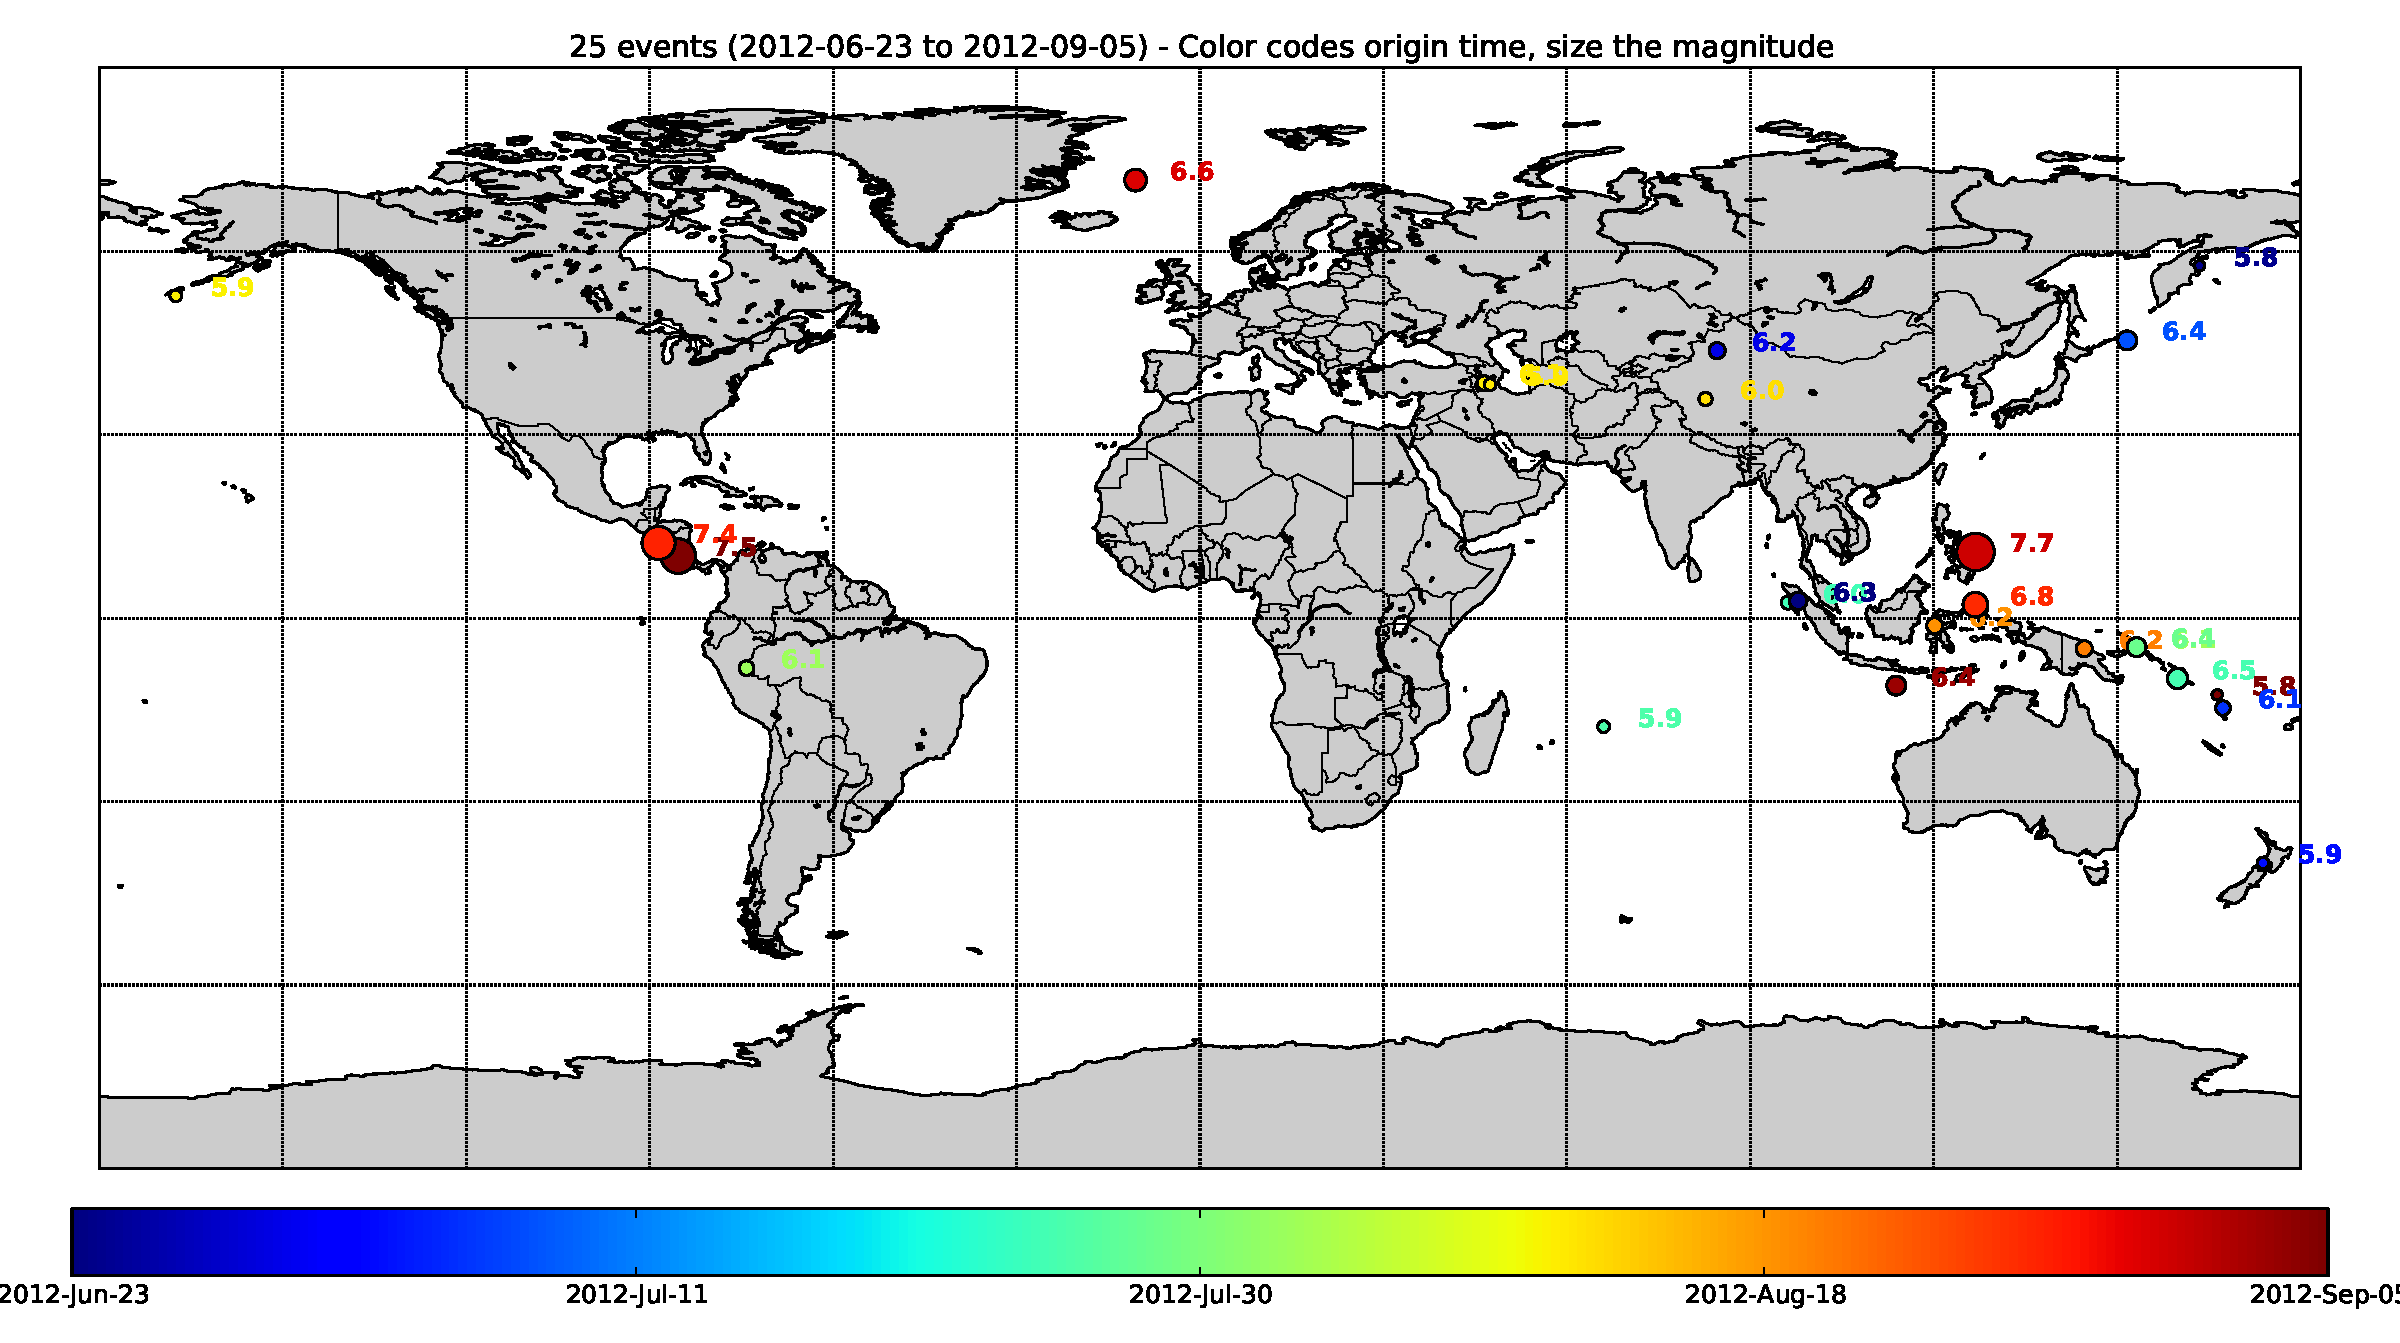
\includegraphics[width=\textwidth]{events.pdf}
\end{frame}

\begin{frame}[fragile, plain]{obspy.core.event - Exercise}
    \begin{itemize}
        \item Read the \textbf{example\_catalog.xml} file.
        \item Plot the events.
        \item Print the resulting Catalog object and filter it, so it only contains events with a magnitude larger then 8.
        \item Now assume you did a new magnitude estimation and want to add it
            to one event. Create a new magnitude object, fill it with some
            values and append it to magnitude list of the largest event.
        \item Write the Catalog as a QuakeML object.
    \end{itemize}
\end{frame}

\begin{frame}[plain, fragile]{}
    \begin{center}
        \textcolor{lmu@darkgreen}{\LARGE{Waveform Plugins}}
    \end{center}
\end{frame}


\begin{frame}[plain, fragile]{Waveform Plugins}
    \begin{itemize}
        \item Read and write support for all waveform formats is handled via plugins.
        \item The following formats are currently supported:
            \begin{itemize}
                \item datamark
                \item gse2
                \item mseed
                \item sac
                \item seg2
                \item segy
                \item seisan
                \item sh
                \item wav
            \end{itemize}
    \end{itemize}
\end{frame}


\begin{frame}[plain, fragile]{Waveform Plugins}
    \begin{itemize}
        \item Format specific header values are stored in the stats object of the Trace, e.g. for files in the MiniSEED format:
    \end{itemize}
\begin{myColorBox}{0.95}{}
\begin{python}
>>> print tr.stats.mseed
AttribDict({"record_length": 512, "encoding": "STEIM1",
    "filesize": 28690432L, "dataquality": "D",
    "number_of_records": 56036L, "byteorder": ">"})
\end{python}
\end{myColorBox}

    \begin{itemize}
        \item Format specific header values are stored in the stats object of the Trace, e.g. for files in the MiniSEED format:
    \end{itemize}

\begin{myColorBox}{0.95}{}
\begin{python}
>>> st = read()
>>> st.write("output_file.mseed", format="mseed",
    "record_length"=1024, "encoding"="STEIM2")
\end{python}
\end{myColorBox}

\end{frame}


\begin{frame}[plain, fragile]{}
    \begin{center}
        \textcolor{lmu@darkgreen}{\LARGE{Retriving Data - ObsPy Clients}}
    \end{center}
\end{frame}

\begin{frame}[plain, fragile]{Clients - Getting waveform data from the web}

\textbf{ObsPy} has clients for \textbf{NERIES}, \textbf{IRIS}, \textbf{ArcLink}, \textbf{SeisHub} and \textbf{Earthworm}.

\begin{myColorBox}{0.95}{}

\begin{python}
>>> from obspy import UTCDateTime
>>> from obspy.arclink.client import Client
>>> client = Client(user="test@obspy.org")
>>> t = UTCDateTime("2009-08-20 04:03:12")
>>> st = client.getWaveform("BW", "RJOB", "", "EH*",
        t - 3, t + 15)
>>> st.plot()
\end{python}

\end{myColorBox}

\begin{itemize}
    \item Similar interfaces for the other clients.
    \item The returned Stream object is already known.
    \item In the end it does not matter if the data originally is from a file or from a webservice.
\end{itemize}

\end{frame}

\begin{frame}[plain, fragile]{Clients - Retrieving other data}
    The webservices are not limited to retrieving waveform data. Depending on the client module used, the available data includes:
    \vspace{2em}
    \begin{itemize}
        \item Event data
        \item Inventory and response data.
        \item Availability information.
        \item \dots
    \end{itemize}
\end{frame}


\begin{frame}[plain, fragile]{obspy.arclink - Retrieving the Instrument Response}
\begin{myColorBox}{0.95}{}
\begin{python}
>>> from obspy import UTCDateTime
>>> from obspy.arclink.client import Client
>>> client = Client(user="test@obspy.org")
>>> dt = UTCDateTime(2009, 1, 1)
>>> paz = client.getPAZ("BW", "MANZ", "", "EHZ", dt)
>>> paz
AttribDict({"poles": [(-0.037004+0.037016j),
                (-0.037004-0.037016j), (-251.33+0j),
                (-131.04-467.29j), (-131.04+467.29j)],
            "sensitivity": 2516778600.0,
            "zeros": [0j, 0j],
            "name": "LMU:STS-2/N/g=1500",
            "gain": 60077000.0})
\end{python}
\end{myColorBox}
\end{frame}


\begin{frame}[plain, fragile]{obspy.arclink - Requesting Inventory Data}
\begin{myColorBox}{0.95}{}
\begin{python}
>>> from obspy import UTCDateTime
>>> from obspy.arclink.client import Client
>>> client = Client(user="test@obspy.org")
>>> inv = client.getInventory("BW", "M*", "*", "EHZ",
        restricted=False, permanent=True,
        min_longitude=12, max_longitude=12.2)
>>> inv.keys()
["BW.MROB", "BW.MANZ..EHZ", "BW", "BW.MANZ", "BW.MROB..EHZ"]
>>> inv["BW"]
AttribDict({"description": "BayernNetz",
            "region": "Germany", ...
>>> inv["BW.MROB"]
AttribDict({"code": "MROB",
            "description": "Rosenbuehl, Bavaria", ...
\end{python}
\end{myColorBox}
\end{frame}


\begin{frame}[plain, fragile]{obspy.arclink - Exercises}
    \begin{enumerate}
        \item Use the obspy.arclink client and request some inventory information of your choice.
        \item Use the gained information to download waveform and response information.
        \item Correct for the instrument and save the file to disc.
        \item (Optional) Use any of the other ObsPy clients. Some have
            additional functionality - refer to the ObsPy documentation for
            more information.
    \end{enumerate}
\end{frame}



\begin{frame}[plain, fragile]{}
    \begin{center}
        \textcolor{lmu@darkgreen}{\LARGE{obspy.signal - Signal Processing Routines}}
    \end{center}
\end{frame}


\begin{frame}[plain, fragile]{}

\footnotesize
\begin{verbatim}
sonic                      cfrequency                fem
array_transff_wavenumber   bwith                     fpm
array_transff_freqslowness domperiod                 em
relcalstack                logbankm                  pm
envelope                   logcep                    tpg
normEnvelope               sonogram                  rdct
centroid                   cosTaper                  fpg
instFreq                   c_sac_taper               eg
instBwith                  evalresp                  pg
xcorr                      cornFreq2Paz              plotTfMisfits
xcorr_3C                   pazToFreqResp             plotTfGofs
xcorr_max                  waterlevel                plotTfr
xcorrPickCorrection        specInv                   recSTALTA
simple                     seisSim                   carlSTATrig
bandpass                   paz2AmpValueOfFreqResp    classicSTALTA
bandstop                   estimateMagnitude         delayedSTALTA
lowpass                    estimateWoodAndersonA...  zDetect
highpass                   konnoOhmachiSmoothing     triggerOnset
envelope                   eigval                    pkBaer
remezFIR                   class PPSD                arPick
lowpassFIR                 rotate_NE_RT              plotTrigger
integerDecimation          rotate_ZNE_LQT            coincidenceTrigger
lowpassCheby2              rotate_LQT_ZNE            utlGeoKm
polarizationFilter         cwt                       utlLonLat
\end{verbatim}
\end{frame}

\begin{frame}[plain, fragile]{Filtering}

\begin{myColorBox}{0.95}{}
\begin{python}
from obspy import read
st = read()
st.filter("highpass", freq=1.0, corners=2, zerophase=True)
\end{python}
\end{myColorBox}

Available filters:
\begin{itemize}
    \item bandpass
    \item bandstop
    \item lowpass
    \item highpass
    \item lowpassCheby2
    \item lowpassFIR (experimental)
    \item remezFIR (experimental)
\end{itemize}



\end{frame}


\begin{frame}[plain, fragile]{Instrument correction}

\begin{myColorBox}{0.95}{}
\begin{python}
from obspy import read
from obspy.signal import cornFreq2Paz
paz_sts2 = {\
    "poles": ...,
    "zeros": [0j, 0j],
    "gain": 60077000.0,
    "sensitivity": 2516778400.0}
paz_1hz = cornFreq2Paz(1.0, damp=0.707)
st = read()
st.simulate(paz_remove=paz_sts2, paz_simulate=paz_1hz)
\end{python}
\end{myColorBox}

\begin{itemize}
    \item The PAZ can also be retrieved from one the webservices, or from a SEED or RESP file.
\end{itemize}

\end{frame}


\begin{frame}[plain, fragile]{}
    \begin{center}
        \textcolor{lmu@darkgreen}{\LARGE{Thanks for your Attention!}}
    \end{center}
\end{frame}


\begin{frame}[plain, fragile]{}
    \begin{center}
        \textcolor{lmu@darkgreen}{\LARGE{Appendix}}
    \end{center}
\end{frame}

\begin{frame}[plain, fragile]{Events - Resource References}
    \begin{itemize}
        \item In QuakeML resources can refer to each other using a unique identifier string.
        \item These connections are preserved in obspy.core.event.
        \item This works across file boundaries assuming all necessary resources have been read before.
    \end{itemize}
\begin{myColorBox}{0.95}{}
\begin{python}
>>> magnitude = event.magnitudes[0]
# Retrieve the associated Origin object.
>>> print magnitude.origin_id
quakeml:eu.emsc/origin/rts/261020/782484
>>> origin = magnitude.origin_id.getReferredObject()
>>> print origin
Origin
  resource_id: ResourceIdentifier(...)
         time: UTCDateTime(2012, 4, 4, 14, 21, 42, 300000)
     latitude: 41.818
    longitude: 79.689
    ...
\end{python}
\end{myColorBox}
\end{frame}



\end{document}
